\iftoggle{title}{
\subsection*{Problem 10}
}{}
\iftoggle{contributions}{
\textit{2023 PHYS 158 Homework 6 question 2}
}{}

\iftoggle{difficulty}{
Difficulty: $\medblackstar \medwhitestar \medwhitestar$
}{}

Consider two solid spheres of radius $R$ with uniformly distributed charge
throughout their volumes. Point $P$ lies on the line connecting the centres of
the spheres and is located at a distance of $0.5R$ from the centre of sphere
1 as shown. If the net electric field at $P$ is zero, what is the ratio $Q_2 /Q_1$ of the
total charge on each sphere?

\begin{center}
    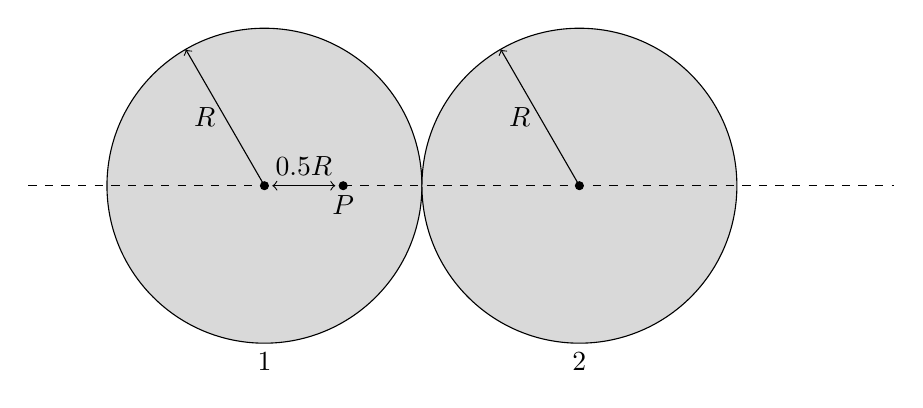
\begin{tikzpicture}
        \draw[fill=gray!30] (0,0) circle (2);
        \draw[fill=gray!30] (4,0) circle (2);
        \draw[fill=black] (0,0) circle (0.05);
        \draw[fill=black] (4,0) circle (0.05);
        \draw[dashed] (-3,0) -- (8,0);
        \draw[->] (0,0) -- (120:2) node[midway, left] {$R$};
        \draw[->] (4,0) -- +(120:2) node[midway, left] {$R$};
        \draw[<->] (0.1,0) -- (0.9,0) node[midway, above] {$0.5R$};
        \draw[fill=black] (1,0) circle (0.05) node[below] {$P$};
        \node[below] at (0,-2) {$1$};
        \node[below] at (4,-2) {$2$};
    \end{tikzpicture}
\end{center}

\iftoggle{solutions}{
\textbf{Solution:}
\begin{center}
    \includegraphics[width=\textwidth]{Images/P10img1.png}
    \end{center}
}{}